\documentclass[aip, amsmath, amssymb, reprint,]{revtex4-2}

\usepackage{graphicx}
\usepackage{dcolumn}
\usepackage{bm}
\usepackage[utf8]{inputenc}
\usepackage[T1]{fontenc}
\usepackage{mathptmx}
\usepackage{etoolbox}

\newcommand\yaq{\texttt{yaq}}

\makeatletter
\def\@email#1#2{%
 \endgroup
 \patchcmd{\titleblock@produce}
  {\frontmatter@RRAPformat}
  {\frontmatter@RRAPformat{\produce@RRAP{*#1\href{mailto:#2}{#2}}}\frontmatter@RRAPformat}
  {}{}
}%
\makeatother
\begin{document}

\preprint{AIP/123-QED}

\title{The yaq Project: \\ A Standard for Scientific Instrumentation}
\author{Kyle F. Sunden}
\author{Daniel D. Kohler}
\author{Kent A. Meyer}
\author{Peter L. Cruz Parilla}
\author{John C. Wright}
\author{Blaise J. Thompson}
\affiliation{
  University of Wisconsin--Madison
}
\email{blaise.thompson@wisc.edu}

\date{\today}

\begin{abstract}

Modern instrumentation development often involves incorporation of many dissimilar hardware peripherals into a single unified instrument.
Increasing availability of modular hardware has brought greater instrument complexity to small research groups.
The flexibility promised to instrument makers by large hardware availability stretches the capability of traditional, monolithic orchestration software.
In many cases, a lack of software flexibility leads creative researchers to feel frustrated, unable to perform experiments they envision.
Herein we describe \yaq{}, a software project defining a new standardized way of communicating with diverse hardware peripherals.
\yaq{} encourages a highly modular approach to experimental software development, which is well suited to address the experimental flexibility needs of complex instruments.
\yaq{} is architected to overcome hardware communication barriers that are insurmountable with typical experimental software.
A large number of hardware peripherals are already supported with tooling available to create more.
The \yaq{} standard enables collaboration among multiple research groups, increasing code quality while lowering development effort.

\end{abstract}

\maketitle

\section{Introduction}

Instrumentation development is a key part of the scientific enterprise.
Novel instruments are typically constructed of many individual components that are both purchased and home-built.
Orchestration software must communicate with each hardware component in the course of a scientific experiment.
This can involve utilization of many interfaces: NI DAQmx\cite{nidaqmx}, SCPI\cite{scpi}, ModBus\cite{modbus}, PICam\cite{picam}, Thorlabs APT\cite{thorlabs_apt}, among many others.
The challenge of integrating all of these interfaces is a frustrating piece of the modern instrument development process.
Weeks can be spent just integrating one new component into an existing project.
In small academic labs, these software interfaces are typically created by student researchers without software development experience.
Student researchers rarely focus on software reusability, and a lack of maintenance and documentation can make such software more difficult to use as time goes on.
Scientists may struggle to rapidly innovate on their experimental design when each hardware addition requires major software development.

Some large user-facilities have addressed interface complexity via the adoption of unified standards, such as EPICS \cite{DalesioLR1991a} or TANGO \cite{AGotz1999TANGOA}.
The unified standards define a network interface for any hardware component.
Orchestration software can target these unified standards for reading and writing hardware state.
Small background services are written to translate the myriad component interfaces into the standard EPICS IOCs and TANGO Devices.
These programs are performant, open source, and have huge libraries of existing hardware interface support, but require expert management to set up and provide descriptions via a separate server program.
In our experience EPICS and TANGO do not scale well to single-investigator lab environments.

As smaller research labs have grown in experimental complexity, many individual labs have created domain-specific orchestration software.
In the last few years, several open source projects by-and-for small-scale experimentalists have grown in popularity\cite{WeberSebastien2021a,Bogdanowicz2022,trspectrometer,Koerner_2019,Campagnola_2014,pymeasure,Giesbrecht_2022,pylablib}.
While this growth is encouraging, many of these are limited by their focus on particular types of hardware or particular experimental domains.
Most small custom research instrumentation continues to rely on monolithic software which has hard-coded interface support for each particular connected device.
These monolithic applications tend to be inflexible and difficult to develop.
%To our knowledge, there are no existing open source projects that attempt to define a unified standard for hardware control of small scale experiments.

We have created a new network-based communication standard for scientific instrumentation, \yaq{}.
This standard borrows the most important ideas from established projects used by large user facilities while retaining the simplicity appropriate for small research labs.
We have built this standard to be self-describing, portable, and reusable wherever possible.
Our primary goal has been to make an interface which simplifies orchestration software development as much as possible.

Here, we discuss the design of the \yaq{} standard in the context of four challenges facing instrument designers.
First, we discuss how particularly challenging hardware interfaces can become seemingly insurmountable barriers to software control.
Next, we discuss how inflexible orchestration software can limit experimental creativity.
Then, we focus on challenges that arise when enhancing or modifying existing instruments with new hardware.
Finally, we discuss the heavy software maintenance burden that many instrument designers face.
In each case, we will highlight how the \yaq{} project is designed to alleviate that challenge.
Several case studies provide a view into the flexible ways that \yaq{} can be applied to perform different scientific experiments.
This paper provides an overview of the concepts and motivations behind \yaq{}.
Refer to the \yaq{} website for a formal specification of the \yaq{} standard.\cite{yaq_fyi}

\section{Hardware Interface Challenges}

In this section we describe the architecture of the \yaq{} framework in light of three major barriers that we have encountered in scientific instrumentation development.
First barrier: Multiple interfaces are used to communicate with each component of the system.
A fully automated system must be able to use all of these interfaces, a daunting task for scientists who do not specialize in software development.
Second barrier: Certain specialty hardware have inconvenient interface requirements.
A camera will only work with an obsolete interface card and drivers for Windows XP.
A data acquisition manufacturer provides an Application Programmer Interface (API) that only works in Python 3.7.
A graduate student wishes to drive several stepper motors using a Raspberry Pi.
Third barrier: Some hardware interfaces are blocking.
A graphical user interface stalls while waiting for a camera to collect data.
Custom orchestration software needs to be closed before the manufacturers configuration software can be used.
A graduate student finds themself needing to master advanced concepts in concurrency in order to orchestrate many motors performantly.

\begin{figure}
	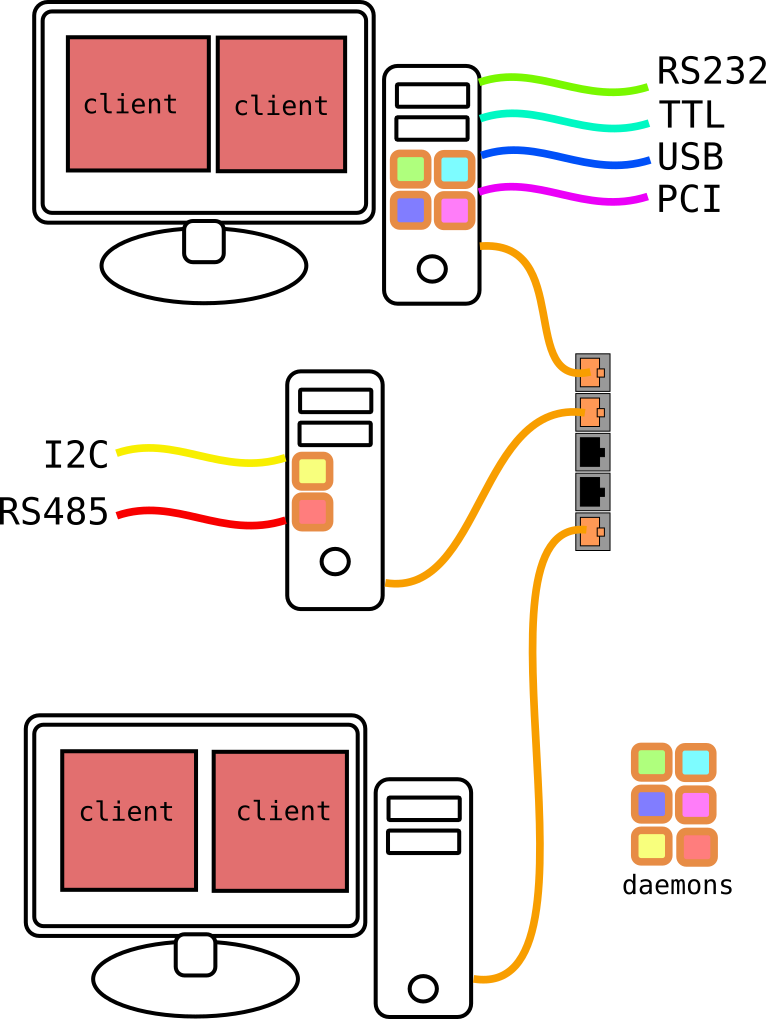
\includegraphics[width=\columnwidth]{figures/network}
\caption{\label{fig:network} Networking diagram}
\end{figure}

Figure \ref{fig:network} diagrams the \yaq{} architecture.
Here, we show three different computers connected via an Ethernet network.
The top and bottom computer are connected to monitors for interactive use while the middle computer is only accessible via the network.
This might represent a complex scientific instrument involving several operator terminals as well as embedded computers.
At the top, a single computer is connected to four hardware peripherals through RS232, TTL, USB, and PCI as indicated by the colored lines.
That same computer is running four separate programs, one for each peripheral.
These small, targeted, programs are managed by the operating system and run in the background.
It is conventional to call such programs ``daemons''\cite{Raymond_1996}.
The middle computer is connected to two additional peripherals, and runs daemons for each.
Besides communicating with the hardware peripheral, each daemon can communicate with other programs, ``clients'',  through the network.
The four client programs shown in Figure \ref{fig:network} can each communicate with all six hardware peripherals shown.
As an example, a client running on the bottom computer could communicate with the RS232 peripheral shown in green via the following path: client $\leftrightarrow$ network switch $\leftrightarrow$ top computer $\leftrightarrow$ daemon $\leftrightarrow$ hardware peripheral.
This powerful architecture can be used on a single computer or used across many networked computers, including fully remote operator interfaces.
This client-server architecture offers similar network capabilities to EPICS and TANGO.
As we will show, usage of standards and the creation of tooling makes this architecture accessible to instrument builders outside of large facilities.

In \yaq{}, communication between daemons and clients is performed over TCP/IP using Apache Avro RPC \cite{AvroSpecification}.
Avro provides an agreed upon standard for efficient serialization of data and method calls from a remote (client) process.
Practically, the \yaq{} interface looks like a collection of methods or functions, which Avro calls ``messages''.
Each message has defined input parameters and output return types.
A sensor might implement a message called ``\texttt{get\_measured}'' which takes no parameters and returns a dictionary mapping channel names to numeric or array data.
A motor would implement a pair of messages for setting and reading back the motor position: ``\texttt{set\_position(float position)} $\rightarrow$ \texttt{null}'' and ``\texttt{get\_position()} $\rightarrow$ \texttt{float}''.
These self describing messages make up the lowest level functionality of the \yaq{} interface.
Each individual communication between client and daemon involves one message being requested by the client and the response returned from the daemon.
Each daemon supports a collection of messages for its unique functionality, called the ``protocol''.

\yaq{} introduces a concept called ``Traits'' which are collections of related messages that are shared among multiple protocols.
Motors implement the ``has-position'' trait, which defines ``\texttt{set\_position}'', ``\texttt{get\_position}'', and ``\texttt{get\_units}''.
Sensors would implement the ``is-sensor'' trait which defines ``\texttt{get\_measured}'', ``\texttt{get\_channel\_names}'', and ``\texttt{get\_channel\_units}''.
Protocols which implement a trait must support all of the messages from the trait.
Importantly, specific protocols can also implement arbitrary additional messages that are not defined by any trait.

The first hardware interface barrier: Multiple incompatible interfaces are used to communicate with each component of the system. % consider making this sentence (and the next paragraph starts) subsection headings
\yaq{} provides a unified TCP/IP interface to all hardware peripherals based on the well-described Avro RPC protocol.
The trait system was introduced in pursuit of our primary goal of easing the client development process.
Clients can trust that protocols that implement a given trait will behave in similar ways.
The standardized \yaq{} interface presents the same set of interactions for client-side scientific code, simplifying the experience of using hardware.

The second hardware interface barrier: Certain specialty hardware have inconvenient interface requirements.
Since \yaq{} enables multiple machines, any hardware requirements can be addressed by putting a machine for that specific hardware on the network.
The Raspberry Pi which drives several stepper motors can be placed onto a private network to communicate with the primary instrument computer using \yaq{}.
Because each \yaq{} daemon is running in its own process, the software environment can be tailored to its needs.
A client running up to date Python 3.10 communicates seamlessly with a daemon running Python 3.7.

The third hardware interface barrier: Some hardware interfaces are blocking.
Monolithic orchestration software often necessitates separate threads for each component hardware interface, a fragile pattern in which small mistakes become both critical and elusive errors.
In \yaq{}, each daemon is only responsible for a single hardware interface.
%Each \yaq{} daemon runs as a separate process (possibly not even on the same machine) and thus many of the hard concurrency problems with communicating with hardware are mitigated.
It is expected that each message call over the \yaq{} interface will return rapidly, ensuring that client applications are not blocked for extended periods of time.
This principle applies even when the message starts an action that might take several seconds to complete, such as homing a motor or initiating a measurement for a sensor.
In these instances, the initial message simply starts the action and returns, with a separate message provided to retrieve results when they exist.
In order to know how long to wait, the ``is-daemon`` trait provides a message called ``is\_busy'' which should return "true" while the long running action is not complete, and "false" once it is finished.
Additionally, multiple clients can communicate with the same daemon simultaneously.
A complex instrument may involve multiple operators watching sensor data in real time, while one program is orchestrating the hardware and recording the data.

\section{Experimental Flexibility}

Existing experimental orchestration software is often highly inflexible.
An experimentalist will spend many hours in lab repeating acquisitions because it is too challenging to add repetition functionality to their software.
A laser lab needs to spend weeks on software development when introducing a single new step into their experimental procedure.
Researchers are disappointed to realize that they are forced to start from scratch when developing software for a similar instrument built with trivially different hardware.

In our view, software inflexibility is a natural consequence of the typical software development practices used by custom instrument builders.
Instrumental software is often built as one monolithic program that does everything from providing a graphical interface, through hardware interfacing, and writing data files.
Such software is typically impossible to debug without access to real hardware, often requiring all of the hardware to be available to simply start the program.
As such, instrumentation software development time is in conflict with valuable data acquisition time.
The hardware interfaces that these programs implement are typically made quickly and without regard to standardization with similar hardware.
The orchestration routines are intimately tied to the particular hardware configuration of one instrument.

Unique experiments will always need custom orchestration and user experience.
We believe that novel instrumentation development naturally and necessarily includes the creation of targeted software.
Developing experimental software is an iterative process tied to the scientific goals of the instrument.
Often experimentalists must apply their specialty scientific knowledge to develop this software.\cite{SegalJudith2005a} % citation does not compile
\yaq{} is architected to encourage better software development practices when creating such programs.
In a \yaq{} context, orchestration code and graphical control interfaces are implemented as clients.
These clients are automatically simpler because they only need to implement the \yaq{} standard and do not need to include the vast array of hardware-specific communication interfaces.
Beyond this, clients can use traits to interact with similar hardware identically.
A client written to perform a two dimensional fluorescence experiment using two Acton monochromators will also work with Horiba monochromators without any modification.

\begin{figure}
\includegraphics[width=\columnwidth]{figures/client_spectrum}
	\caption{  \label{fig:foundation} \yaq{} scales from simple scripts to integrations with featureful frameworks.}
\end{figure}

A \yaq{} client can scale in complexity from a small, lightweight script all the way to a sophisticated graphical program, as shown in Figure \ref{fig:foundation}.
At the bottom, we represent the most lightweight interface to \yaq{}, Python scripting.
\texttt{yaqc}\cite{yaqc} is a Python client which is excellent for using in scripts or any other Python program.
The code shown creates three client objects which could be used directly through an interactive Python prompt or in a reusable script.
Each client object provides Python methods for each Avro message specified by the associated protocol.

In the middle, the same three hardware peripherals are represented in an interactive, graphical form.
\texttt{yaqc-qtpy}\cite{yaqc-qtpy} is a graphical application which builds interactive controls based on traits for any conceivable \yaq{} protocol.
The self describing \yaq{} interface is used to provide graphical elements for the most commonly used messages.
This is an invaluable tool which provides a ``free'' graphical user interface (GUI) to any daemon.

At the top, we show several features associated with the integration between \yaq{} and the Bluesky project\cite{AllanDanielB2019a}.
Bluesky provides a powerful orchestration layer for conducting and recording data for a wide variety of experimental procedures.
Shown in Figure \ref{fig:foundation}, we see one such GUI for parameterizing a Bluesky procedure and a representation of the resultant data.
\texttt{yaqc-bluesky}\cite{yaqc-bluesky} provides a bridge to the Bluesky ecosystem.
Similar translation layers could be built for a variety of orchestration layers such as PyMoDAQ\cite{WeberSebastien2021a}, Instrumental\cite{Bogdanowicz2022}, or TRSpectrometer\cite{trspectrometer}.

All three types of clients represented in Figure \ref{fig:foundation} have been shown addressing the same three hardware peripherals.
All types of clients can be used simultaneously to interact with the same instrument in different modes.
Client sophistication can be introduced naturally, as novel experiments are tested and refined.
Different clients can specialize for different requirements of a custom instrument.
For example, \texttt{yaqc-qtpy} can provide a quick interface for setting and viewing hardware positions while Bluesky can focus on experimental data acquisition.

The Landis Group at UW-Madison is currently working on a new type of flow reactor: the Wisconsin Quench Kinetics Reactor (WiQK).
This reactor incorporates several computer-controlled valves and syringe pumps as well as various sensors.
The set of hardware peripherals is rapidly changing as researchers continue to test and refine their design.
Only a few researchers are actively using the reactor during this prototyping stage.
These researchers are experimentalists who have limited background in software development.
The Landis Group has written basic Python scripts to orchestrate hardware for their reactor.
These lightweight scripts can be extensively refactored by the experimentalists as the hardware and orchestration strategy changes dramatically during WiQK development.
This approach ensures that the Landis Group is not slowed down by complex, inflexible orchestration software.
Once the reactor is complete, more sophisticated graphical clients will be created to accommodate end users who were not involved as the reactor was built.

The Wright Group at UW-Madison needs to orchestrate a large variety of hardware in multidimensional scans for their complex spectroscopy experiments \cite{MukamelShaul2000a, WrightJohnCurtis2011a}.
This need for exquisite hardware control has resulted in several prior attempts at ``home-built'' orchestration software \cite{CarlsonRogerJohn1988a, MeyerKentAlbert2004b, KainSchuyler2017a, ThompsonBlaiseJonathan2018a}.
Now, using \yaq{}, the Wright Group has been able to move to Bluesky rather than inventing their own sophisticated control software ``from scratch''.
The Wright Group uses simulated hardware to enable client development away from the active laboratory computers.
This allows Wright Group researchers to create polished client interfaces without interrupting  ongoing experiments.
Clients developed by the Wright Group have proved flexible enough to be used on four laser systems, each with different complements of hardware.
Moving forward, the Wright Group will spend less energy developing control software and more energy developing creative spectroscopy experiments.

\section{Incorporating New Hardware}

In a \yaq{} context, new hardware can be incorporated into an instrument through the addition of a new daemon.
The \yaq{} architecture simplifies hardware interface development in several ways.
First, because daemons are separate and portable programs, the development effort can be spread across the community of \yaq{} users.
Often, researchers can download an existing daemon rather than writing a new one.
Second, \yaq{} daemon development can be performed separated from the particulars of any individual client.
Often, this means that initial hardware enablement work can be done on a researchers personal machine before the new hardware peripheral is installed in the instrument.
Third, when developing trait-compliant protocols, it becomes easy to design and fully test your hardware interface.
Traits are unambiguous and well-described, making an obvious target for development.
Tooling exists to verify full trait compliance, for example you can use \texttt{yaqc-qtpy} to provide a graphical program to interact with your hardware immediately.
Finally, as discussed in Section II, \yaq{} gives you options to design using remote hardware or unusual interfaces when necessary.

We have created several tools to aide in daemon development.
First, a Python library, \texttt{yaqd-core}\cite{yaqd-core-python}, which implements shared functionality.
Second, \texttt{yaq-traits}\cite{yaq-traits} is a command line application which allows the description of messages provided by a \yaq{} protocol to be written in a human-readable fashion and translated into a more fully described machine readable format.
The format it generates is an important part of how \yaq{} protocols are self describing.
This shields developers from the details of Apache Avro, which can be somewhat esoteric.

\begin{figure}
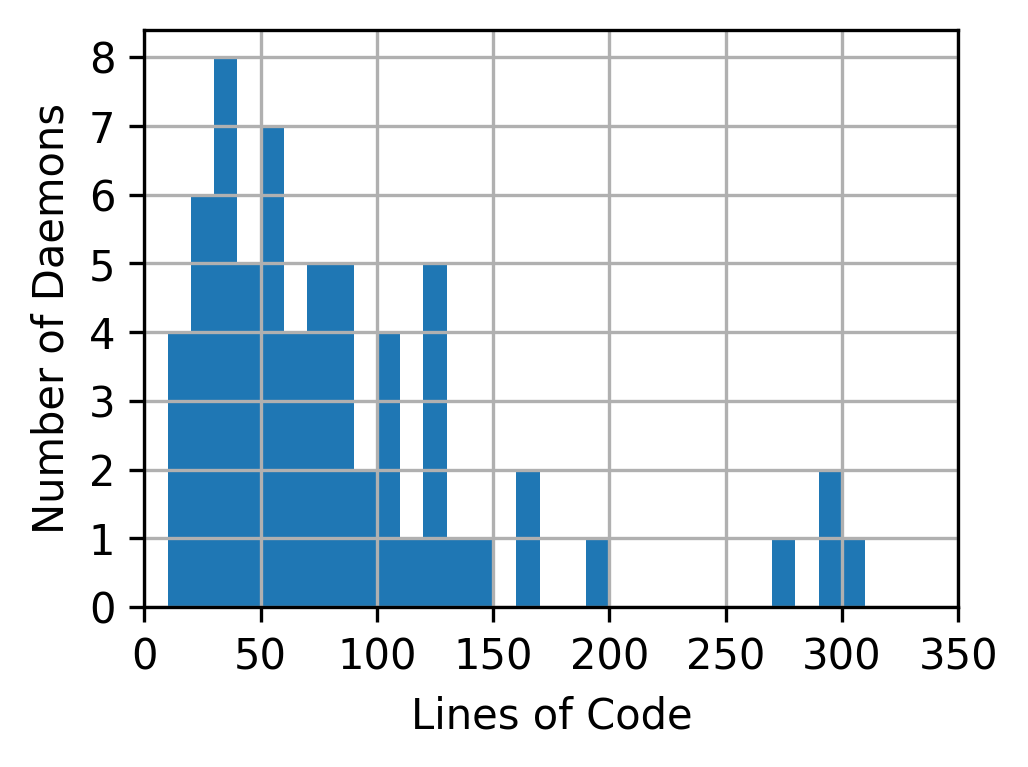
\includegraphics[width=\columnwidth]{figures/lines_histogram},
	\caption{  \label{fig:histogram} Histogram of the number of lines for each implemented daemon.
	Some daemons are implemented in ways that share code, resulting in apparent line counts less than 10.
	For example, the Thorlabs APT\cite{thorlabs_apt} motor implementation supports at least eight different daemons with each specifying only a handful of constants.
	These are extreme examples which are not representative of most hardware interfaces, so we omit them here. % it's not clear to me why these instances are not included (and scaled down???) It is a _feature_ not a bug that one can implement motor support with tiny amounts of code.
	}
\end{figure}

Figure \ref{fig:histogram} shows the distribution of unique lines of Python code written to implement each of the daemons in our current ecosystem.
While lines of code is an imperfect metric, we use it here to represent the amount of work required to create a daemon for a new hardware peripheral.
Most interfaces, such as Brooks MFC\cite{yaqd-brooks-mfc}, have been implemented in fewer than 100 lines of Python code.
Even the most complicated daemons are implemented in about 300 lines.
Implementing \yaq{} daemons using Python is enabled through our own tooling mentioned above and the large and growing ecosystem of hardware interface tooling libraries that Python now provides\cite{}.
In our experience, the process of creating a new daemon involves about a day of work after communication with the hardware using Python is well understood.
There are currently 70 daemons in the yaq project supporting at least 50 kinds of hardware, noting that some daemons support the same hardware and others are software only.
Because \yaq{} is standards based, anyone can design and publish new daemons extending our hardware support.
A living list of all daemons and supported hardware can be found on the \yaq{} website.\cite{}

The Stahl Group at UW-Madison created a custom reactor which monitors gasses being produced or consumed in the reaction head-space.  \cite{SalazarChaseA2021a}
This reactor incorporates a collection of sensitive pressure transducers and a single heating process value under computer control.
\yaq{} daemons are used to interface with each sensor and the heater controller.
Recently, experimentalists have been attempting reactions involving smaller, slower, pressure changes.
A fundamental flaw in the initial analog to digital converter board was revealed by these attempts.
As a result, a new digitizer has been purchased.
This new digitizer will be incorporated into the existing reactor without modifying the existing graphical user interface and data recording program, minimizing downtime.

\section{Technical Debt}

Years after the original researchers leave, large monolithic acquisition programs become unknowable, undocumented, and unmaintained.
A graduate student discovers a hard-coded conversion factor that is incorrect years after implementation.
Scientists resort to sourcing a replacement for an old, broken oscilloscope due to their reliance of their software on that particular interface while newer, cheaper oscilloscopes are readily available.
A graduate student is forced to meticulously reverse engineer the LabVIEW codebase that they inherited in order to understand the details of their experiment.
Software developers refer to the extra effort required to modify or fix large unmaintained codebases as ``technical debt''.\cite{}
Technical debt grows especially fast in academic environments where graduate students are involved in projects for a limited time.

The \yaq{} approach favors many small single-purpose applications above large monolithic ones.
For daemons, the purpose of each application is obvious and unambiguous.
There is a strict, well defined interface which explicitly limits the kinds of interactions that are provided to the hardware, thus limiting opportunity for unintended consequences.
The lack of hardware interface code makes \yaq{} clients much simpler and easier to describe and maintain.
Tools like \texttt{yaqd-fakes}\cite{yaqd-fakes} allow clients to be tested and improved outside of their instrument, including the possibility of fully automated testing.
Simple, script-based clients written using the expressiveness of Python can be read and understood in hours rather than weeks.
Integrations with communities like Bluesky offer powerful features which are actively maintained across many institutions.

In \yaq{}, each component of an instrument can be developed and distributed separately.
For example, two different instruments might happen to use the same temperature sensor.
Because the temperature sensor daemon is its own independent program, both instruments can benefit from the same daemon.
The growing ``ecosystem'' of \yaq{} daemons make future instruments easier and easier to develop.
Growing this ecosystem is a collaborative effort where many \yaq{} users create portable daemons that they need and share them with the community where they will be used and improved.

Software documentation is famously difficult and thankless work.
\yaq{} attempts to automate daemon documentation as much as possible.
Our website, https://yaq.fyi, automatically builds generated reference pages for all known protocols.
These pages are automatically updated when new versions are published.

\yaq{} is open source software.
Anyone can view, install, edit, and suggest changes to our growing collection of daemons and clients.
Furthermore, anyone can create their own totally-custom client or daemon software separately by following the specified \yaq{} standard.
Thirteen individuals have contributed code to the development of \yaq{}.
Open-source development can be a powerful approach for research communities looking to share software-development and maintenance burdens. \cite{CohenJeremy2021a}
It is our hope that a vibrant open-source community will form around \yaq{}.
While open-source development is not a panacea \cite{NowogrodzkiAnna2019a}, we hope that by maintaining a distributed development strategy with a strict focus on only hardware interfaces the \yaq{} project might prove sustainable.

\section{Conclusion}

The \yaq{} project defines a new general-purpose standard for hardware control in the context of scientific instrumentation.
This standard has some of the powerful features of facility-scale standards while remaining simple enough for feasible implementation and maintenance in small research labs.
We have shown how this approach alleviates common problems through discussion and case studies.
Designing around self-describing protocols is a productive approach that has great promise in scientific software development.

\begin{acknowledgments}
  TODO
\end{acknowledgments}

\section*{Data Availability Statement}

Data sharing is not applicable to this article as no new data were created or analyzed in this study.

\section*{References}
% all yaq,yaqc,and yaqd citations have an unfilled "()" in them...
\nocite{*}
\bibliography{references}

\end{document}
